\documentclass[18pt,compress,ngerman,utf8,t]{beamer}
\usepackage{etex}
\usepackage[ngerman]{babel}
\usepackage{graphicx}
\usepackage[export]{adjustbox}
\usepackage{multicol}


\usetheme[numbering=fraction, progressbar=frametitle]{metropolis}


\date{\today}
\institute{Student of Rationality}
\graphicspath{ {./template/} {./lesswrong/graphics/} }
% \titlegraphic{\vspace{4cm} \hspace{9cm} \includegraphics[height=2cm]{template/Logo-LessWrong.png}}

\title{How to be less wrong}
\author{Felix Karg}

\newif\ifEnglish
\Englishfalse
% \Englishtrue

\AtBeginSection[]
{
    \large
    \begin{frame}{Inhalt}
        \begin{multicols}{2}
            \tableofcontents[currentsection]
        \end{multicols}
        \clearpage
    \end{frame}
}

\AtBeginSubsection[]
{
    \large
    \begin{frame}{Inhalt}
        \begin{multicols}{2}
            \tableofcontents[currentsection,currentsubsection]
        \end{multicols}
        \clearpage
    \end{frame}
}

% \vspace{0.1cm}



\newcommand{\code}[1]{
    \begin{center}
    \setlength{\fboxrule}{1pt}
    \setlength{\fboxsep}{8pt}
        {\fbox{\parbox{0.81\textwidth}{#1}}}
   \end{center}
}




\begin{document}

\maketitle

% multicols from:
% https://tex.stackexchange.com/questions/24343/splitting-toc-into-two-columns-on-single-frame-in-beamer

%%%%%%%%%%%%%%%%%%%%%%%%%%%%%%%%%%%%%%%%%%%%%%%%%%%%%%%%%%%%%%%%%%%%%%%%%%%%%%%%%%%%%%%%%%%%%%%%%%%%%%%%%%%%%%%%%%%

\begin{frame}{Inhalt}
    \Large
    \begin{multicols}{2}
        \tableofcontents[hidesubsections]
    \end{multicols}
    % \clearpage
\end{frame}




%%%%%%%%%%%%%%%%%%%%%%%%%%%%%%%%%%%%%%%%%%%%%%%%%%BEGINNING%%%%%%%%%%%%%%%%%%%%%%%%%%%%%%%%%%%%%%%%%%%%%%%%%%%%%%%%
% \ifEnglish


\begin{frame}[c]{What is Rationality about?}
    Testframe
\end{frame}

% \begin{frame}[standout]
%     Rationality is {\emph about} winning.
% \end{frame}


\else

\section{Was ist Rationalität?}

\begin{frame}[c]{Was ist Rationalität?}
    \Large
    Grob:
    \newline
    \begin{itemize}
    \pause
    \item Die Welt verstehen    \only<3->{(Epistemic Rationality)}
    \newline
    \pause
    \pause
    \item Ziele erreichen       \only<5->{(Instrumental Rationality)}
    \newline
    \end{itemize}
    \pause
    \pause
    Kurz: Rationalität entwickelt unsere Entscheidungen bezüglich Denken und Handeln weiter.
\end{frame}


\begin{frame}[c]{Was ist Rationalität?}
    \Large
    Nutzen von hilfreichen Erkenntnissen aus anderen Bereichen, z.B.:
    \begin{itemize}
    \pause
    \item Bayes' Theorem        \only<3->{(Statistik)}
    \pause
    \pause
    \item Modelle               \only<5->{(Philosophie)}
    \pause
    \pause
    \item Occams Rasiermesser   \only<7->{(Entscheidungstheorie)}
    \pause
    \pause
    \item System I/II           \only<9->{(Kognitionswissenschaften)}
    \pause
    \pause
    \item Rätselhafte Antworten \only<11->{(...)}
    \end{itemize}
\end{frame}

% Wertetheorie, Erkenntnistheorie, Metaphysik

\begin{frame}[c]{Was tun mit den Erkenntnissen?}
    \Large
    \pause
    Optimieren von ...
    \begin{itemize}
    \pause
    \item Strukturen
    \pause
    \item Denkprozessen
    \pause
    \item Verfahrensprozessen
    \pause
    \item ...
    \end{itemize}
\end{frame}





\fi

\ifEnglish


\begin{frame}[c]{What is Rationality about?}
    Testframe
\end{frame}

% \begin{frame}[standout]
%     Rationality is {\emph about} winning.
% \end{frame}


\else

\section{Was ist Rationalität?}

\begin{frame}[c]{Was ist Rationalität?}
    \Large
    Grob:
    \newline
    \begin{itemize}
    \pause
    \item Die Welt verstehen    \only<3->{(Epistemic Rationality)}
    \newline
    \pause
    \pause
    \item Ziele erreichen       \only<5->{(Instrumental Rationality)}
    \newline
    \end{itemize}
    \pause
    \pause
    Kurz: Rationalität entwickelt unsere Entscheidungen bezüglich Denken und Handeln weiter.
\end{frame}


\begin{frame}[c]{Was ist Rationalität?}
    \Large
    Nutzen von hilfreichen Erkenntnissen aus anderen Bereichen, z.B.:
    \begin{itemize}
    \pause
    \item Bayes' Theorem        \only<3->{(Statistik)}
    \pause
    \pause
    \item Modelle               \only<5->{(Philosophie)}
    \pause
    \pause
    \item Occams Rasiermesser   \only<7->{(Entscheidungstheorie)}
    \pause
    \pause
    \item System I/II           \only<9->{(Kognitionswissenschaften)}
    \pause
    \pause
    \item Rätselhafte Antworten \only<11->{(...)}
    \end{itemize}
\end{frame}

% Wertetheorie, Erkenntnistheorie, Metaphysik

\begin{frame}[c]{Was tun mit den Erkenntnissen?}
    \Large
    \pause
    Optimieren von ...
    \begin{itemize}
    \pause
    \item Strukturen
    \pause
    \item Denkprozessen
    \pause
    \item Verfahrensprozessen
    \pause
    \item ...
    \end{itemize}
\end{frame}





\fi


% \section{Examples}

\begin{frame}[c]
     Here a citation: \cite{benchcpp}
\end{frame}

\begin{frame}[c]{Example slide}
    \Large
    \begin{itemize}[<+->]
        \item First Element
        \item Second Element
        \item Third Element
    \end{itemize}
\end{frame}

\begin{frame}[c]{Other example slide}
    \Large
    \begin{itemize}[<+(1)->]
        \item First Element
        \item Second Element
        \item Third Element
    \end{itemize}
\end{frame}

\begin{frame}[c]{Yet another example slide}
    \Large
    \begin{itemize}
        \item First Element
            \pause
        \item Second Element
            \pause
        \item Third Element
    \end{itemize}
\end{frame}









% \ifEnglish
%%%%%%%%%%%%%%%%%%%%%%%%%%%%%%%%%%%%%%%%%%%%%%%%%%%%%%%%%%%%

\section{Predictably Wrong}





%%%%%%%%%%%%%%%%%%%%%%%%%%%%%%%%%%%%%%%%%%%%%%%%%%%%%%%%%%%%
\else
%%%%%%%%%%%%%%%%%%%%%%%%%%%%%%%%%%%%%%%%%%%%%%%%%%%%%%%%%%%%

\section{Vorhersagbar Falsch}

\begin{frame}[c]{Unwahrscheinliche Details}
    
\end{frame}





%%%%%%%%%%%%%%%%%%%%%%%%%%%%%%%%%%%%%%%%%%%%%%%%%%%%%%%%%%%%
\fi


% \ifEnglish
%%%%%%%%%%%%%%%%%%%%%%%%%%%%%%%%%%%%%%%%%%%%%%%%%%%%%%%%%%%%

\section{Occam's Razor}

\begin{frame}[c]{Occam's Razor - General Description}
    Usually something like this: ...
\end{frame}



%%%%%%%%%%%%%%%%%%%%%%%%%%%%%%%%%%%%%%%%%%%%%%%%%%%%%%%%%%%%
\else
%%%%%%%%%%%%%%%%%%%%%%%%%%%%%%%%%%%%%%%%%%%%%%%%%%%%%%%%%%%%

\section{Occam's Rasiermesser}

\begin{frame}[c]{Occam's Rasiermesser - Allgemeine Beschreibung}
    Üblicherweise sinngemäß so: ...
\end{frame}


%%%%%%%%%%%%%%%%%%%%%%%%%%%%%%%%%%%%%%%%%%%%%%%%%%%%%%%%%%%%
\fi


% 
\begin{frame}[c]{Geländeplan}
    % trim = l b r t
    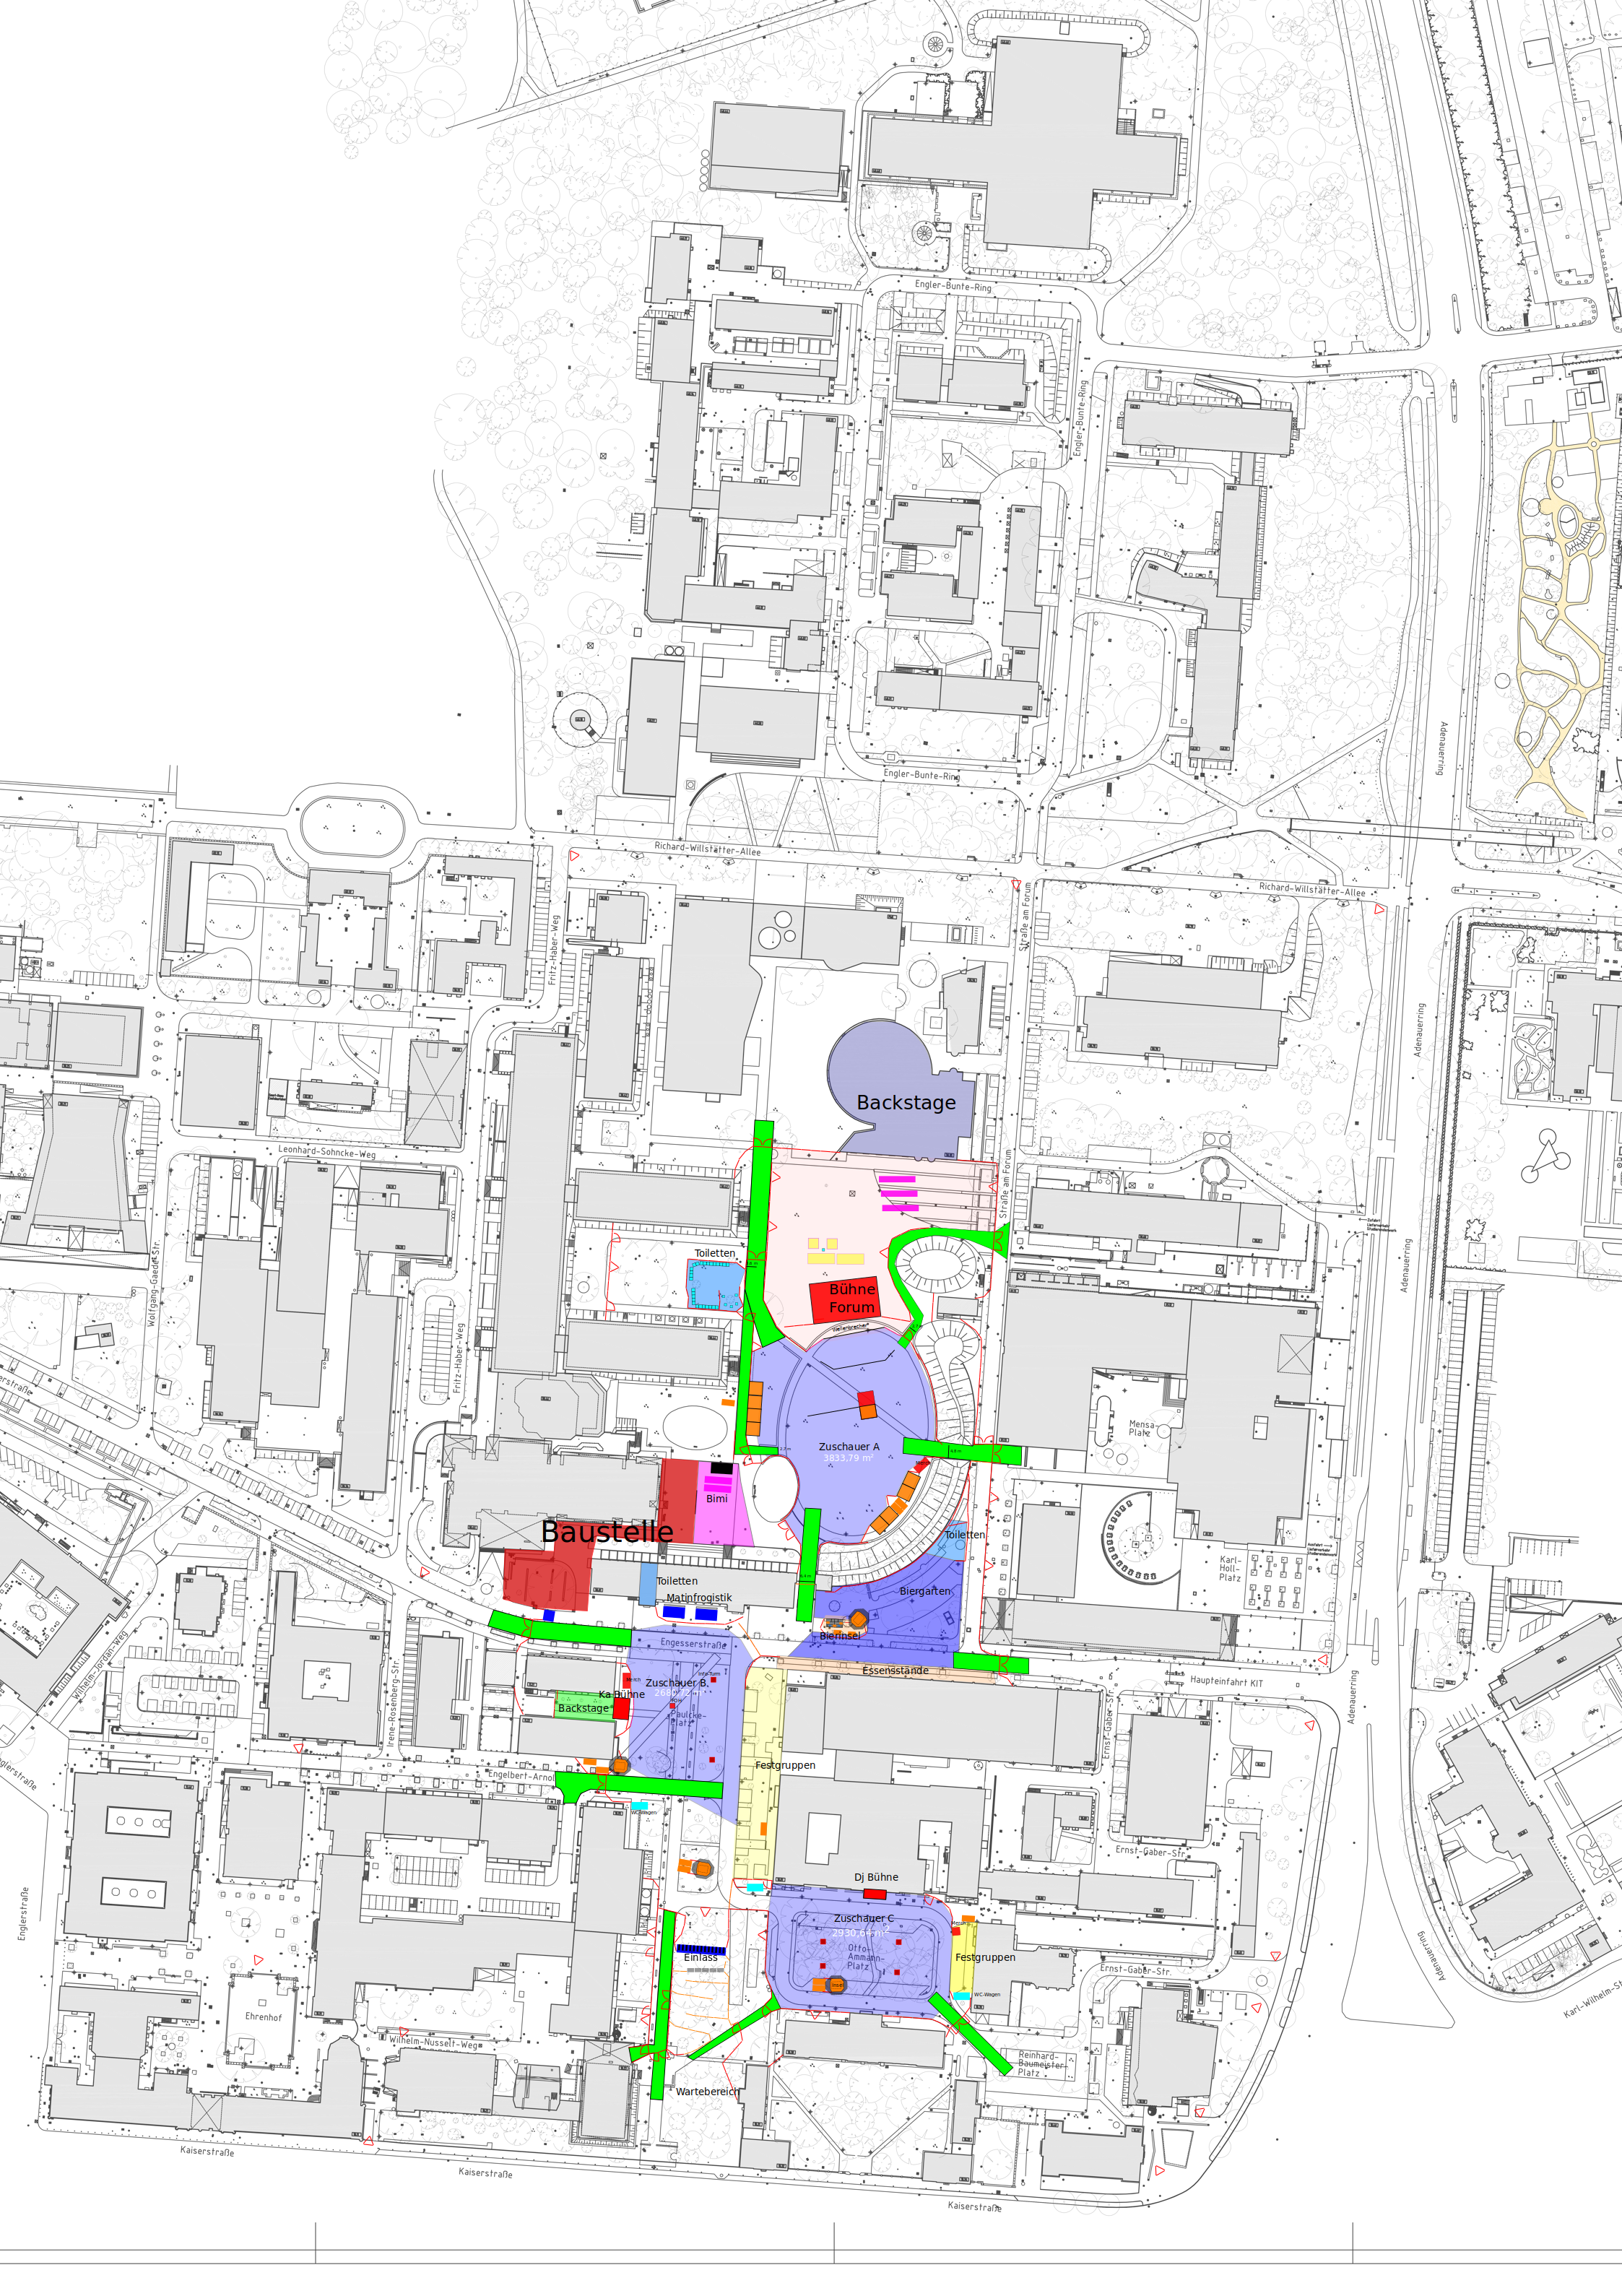
\includegraphics[height=0.95\textheight,clip,trim = 500 150 700 1400]{Plan_Freitag}
\end{frame}





%%%%%%%%%% END %%%%%%%%%%
% \ifEnglish
%%%%%%%%%%%%%%%%%%%%%%%%%%%%%%%%%%%%%%%%%%%%%%%%%%%%%%%%%%%%

\section{Sources}

\begin{frame}[c]
    
\end{frame}



%%%%%%%%%%%%%%%%%%%%%%%%%%%%%%%%%%%%%%%%%%%%%%%%%%%%%%%%%%%%
\else
%%%%%%%%%%%%%%%%%%%%%%%%%%%%%%%%%%%%%%%%%%%%%%%%%%%%%%%%%%%%


%%%%%%%%%%%%%%%%%%%%%%%%%%CITES%%%%%%%%%%%%%%%%%%%%%%%%%%%%%
\section{Quellen}

%%%%%%%%%%%%%%%%%%%%%%%%%%CITES%%%%%%%%%%%%%%%%%%%%%%%%%%%%%
\begin{frame}[c,fragile,allowframebreaks]{Quellen}
    Die Folien sind zu finden unter: \newline
    \url{https://github.com/fkarg/things-to-talk-about/tree/master/lesswrong}
    \newline
    \newline
    Das Forum, mit diesen und sehr viel mehr Themen: \newline

% 
% 
%     Das Buch, aus dem ich den Vortrag gebastelt hab:
% 
    \beamertemplatearticlebibitems
    \begin{thebibliography}{10}
    \bibitem{Less Wrong}
            {\bf Less Wrong}
            \newblock \url{http://lesswrong.com/}

%     \beamertemplatebookbibitems
%     \bibitem{Richard Rumelt}
%         Richard Rumelt
%         \newblock {\em Good Strategy / Bad Strategy}.
%         \newblock The Difference and Why It Matters \\
%                   ISBN: 978-1-78125-154-6
%     \beamertemplatearticlebibitems
%     \bibitem{Lesswrong}
%         Lesswrong
%             \newblock {\em Expecting short Inferential Distances}
%             \newblock \url{http://lesswrong.com/lw/kg/expecting\_short\_inferential\_distances/}
%     \bibitem{Lesswrong}
%         Lesswrong
%             \newblock {\em Cached Thoughts}
%             \newblock \url{http://lesswrong.com/lw/k5/cached\_thoughts/}
%     \bibitem{Zenhabits}
%         Zenhabits
%             \newblock {\em say No so you can say YES}
%             \newblock \url{https://zenhabits.net/say-yes/}
% 
%     \bibitem{Wikiquote}
%         Fukuzawa Yukichi
%             \newblock {\em Wikiquote}
%             \newblock \url{https://en.wikiquote.org/wiki/Fukuzawa\_Yukichi}
% 
%     \bibitem{SpaceX}
%         SpaceX
%             \newblock {\em SpaceX}
%             \newblock \url{http://www.spacex.com/}
% 
%    \bibitem{Wihipedia}
%        Wikipedia
%            \newblock {\em Proton-M}
%            \newblock \url{https://en.wikipedia.org/wiki/Proton-M}
%    \bibitem{Wikipedia}
%        Wikipedia
%            \newblock {\em Ariane 5}
%            \newblock \url{https://en.wikipedia.org/wiki/Ariane\_5}
%    \bibitem{Wikipedia}
%        Wikipedia
%            \newblock {\em Delta IV Heavy}
%            \newblock \url{https://en.wikipedia.org/wiki/Delta\_IV}
   \end{thebibliography}
    % required the allowframebreaks for longer lists

\end{frame}



%%%%%%%%%%%%%%%%%%%%%%%%%%%%%%%%%%%%%%%%%%%%%%%%%%%%%%%%%%%%
\fi



% generally don't forget: after 20min of talk, 5min short recap + exercise.




% conter deklarieren funktioniert so:
% \newcounter{official}
% \setcounter{official}{\value{page}}

%%%%%%%%%%%%%%%%%%%%%%%%%%%%%%%%%%%%%%%%%%%%%%%%%%%%%%%%%%%%%%%%%%%%%%%%%%%%%%%%%%%%%%%%%%%%%%%%%%%%%%%%%%%%%%%%%%%


\end{document}
